\documentclass[a4paper]{article}

%% Language and font encodings
\usepackage[english]{babel}
\usepackage[utf8x]{inputenc}
\usepackage[T1]{fontenc}

%% Sets page size and margins
\usepackage[a4paper,top=3cm,bottom=2cm,left=3cm,right=3cm,marginparwidth=1.75cm]{geometry}

%% Useful packages
\usepackage{amsmath}
\usepackage{graphicx}
\usepackage{textpos}
\usepackage{float}
\usepackage[colorinlistoftodos]{todonotes}
\usepackage[colorlinks=true, allcolors=black]{hyperref}
\usepackage[numbered,framed]{matlab-prettifier}

\title{\vspace*{2cm}1.1 Golden Section Search for the Mode of a Function\vspace*{-1.5cm}}
\date{}

\begin{document}
\maketitle

\begin{textblock*}{100mm}(0cm,-5.5cm)
\Huge 1.1
\end{textblock*}

\section*{Question 1}
Below are the equations from the golden section search (GSS).
\begin{gather}
(y-a)/(b-a) = (\sqrt[]{5}-1)/2 \\
b-x = y-a
\end{gather}
Using equations (1) and (2) below is an algebraic proof that the subinterval in which the mode is deduced to lie after an iteration of GSS is divided in golden section by the point in its interior.
\begin{align*}
\frac{y-a}{x-a} &= \frac{y-a}{y-b} \\
&= \frac{(a+(a-b)*\phi^{-1})-a}{(a+(a-b)*\phi^{-1})-b} \\
&= \frac{1}{\phi +1} = \phi
\end{align*}

\subsection*{Programming Task}
I wrote program Question\textunderscore2.m to implement the golden section search. It begins by prompting the user to enter the starting interval boundaries and the required precision and then returns the location of the mode, the accuracy of the determined value and the number of iterations used to achieved the desired accuracy.
\renewcommand{\labelenumi}{\roman{enumi}}
\begin{enumerate}
   \item
   		My program deals with the possibility that $f(x) = f(y)$ on one or more iterative steps by checking explicitly for such an occurrence on every iteration. It uses an if-elseif-elseif statement to determine whether $f(x)>f(y)$ , $f(x)<f(y)$ or $f(x)=f(y)$. In the latter case it shrinks the interval of search to $[x,y]$ and then selects two new internal points using equations (1) and (2).
   \item
   		When locating the second internal point in any given iteration it is preferable to use equation (2) instead of equation (1) because it requires less elementary numerical operations ($+,-,\times,\div$) and so runs faster. Equation (2) uses only addition and subtraction while Eqn (1) uses three operations.
   \item
   		My program assumes that the given function is unimodal according to the definition specified in the project but it doesn't assume the nature of the mode. Therefore it begins by determining whether the mode is a maxima, minima or if in fact the function is strictly monotonic. It does this by estimating the gradients at the endpoints and comparing their signs. In the case that both gradient estimates are of the same sign then the program deduces that the function must be monotonic on the range and so outputs this information and the two end-points.
\end{enumerate}

\pagebreak
\section*{Question 2}
Setting my program to look at $f(x) = 1+x+x^2-4x^4$ and inputting a starting interval of $[0,1]$ with an accuracy of 0.0001 it produces the output below:
\begin{verbatim}
Mode located at: 5.000000e-01 
Accuracy: +/- 8.653514e-05 
Number of iterations of golden section search: 18
\end{verbatim}

\section*{Question 3}
Golden section search algorithm
\[ \frac{y-a}{b-a} = \phi^{-1} \qquad b-x = y-a \]
Alternative algorithm
\[ x-a=\frac{1}{3}(b-a) \qquad y-a = \frac{2}{3}(b-a) \]
\\ \\
The most time-consuming part of either algorithms is likely evaluating the function in question. Particularly because the function will likely be a complicated one otherwise analytic methods would have been used instead of computational methods.
\\ \\
A comparison of the two algorithms can be made by considering the elementary numerical operations required to locate the second internal point in each iteration. For GSS using  $b-x=y-a$  involves two elementary operations to calculate $x$ from $y$ or vice versa. For the alternative algorithm both equations  $x-a=\frac{1}{3}(b-a)$  and  $y-a = \frac{2}{3}(b-a)$  involve three operations to calculate $x$ from $y$ or vice versa. Therefore GSS uses fewer numerical operations compared with the alternative algorithm.
\\ \\
In addition, every iteration of GSS reduces the range containing the mode to $\phi^{-1} \approx 0.618$ of it's original length while the alternative algorithm removes only a third, taking the range to $2/3 \approx 0.667$ of its original length. This means the alternative algorithm will take more iterations to reach the same accuracy than GSS. From the calculation below the alternative algorithm will take approximately 19$\%$ more iterations.
\begin{align*}
\phi^{-1} &= \Big(\frac{2}{3}\Big)^n \\
n &= -\frac{\ln{\phi}}{\ln{2/3}} \\
n &\approx 1.19
\end{align*}
Overall, combining both these observations, this means that the alternative algorithm would use appropriately $3/2 \times n \approx 1.78$ times as many numerical operations as GSS. 

\section*{Question 4}
Every iteration of GSS reduces the width of the search interval  $[a,b]$  containing the mode to $(b-a)\times\phi^{-1}$. Therefore the accuracy attainable is limited by the number of iterations it is possible to carry out which is limited by the precision to which $f(x)$ can be evaluated. As soon as the precision to which $f(x)$ can be calculated grows larger than the difference in $f(x)$ across the search interval then it is not possible to proceed with the algorithm.

\pagebreak
\section*{Question 5}
Suppose the mode were located at $x$ with an accuracy of $\pm h$ where $h$ is sufficiently small then the accuracy of the height of the mode would be dependent on the derivative of the function at the point $x$. The accuracy would be approximately $ \pm hf'(x) $
\[ f(x \pm h) = f(x) \pm hf'(x) + o(h^2) \]

\section*{Question 6}
For this question I wrote program Question\textunderscore6.m. It takes no input as the restricted variables, $l$, $r$ and $R$, are hard-coded in. It returns the corresponding optimal values of $d$ and $\theta$. Below is the output upon running:
\begin{verbatim}
The optimum values are 
 theta = 4.635919e-01 rad 
     d = 2.172385e+01 cm 
\end{verbatim}

\renewcommand{\labelenumi}{\roman{enumi}}
\begin{enumerate}
\item
	In order to play the entirety of the vinyl record the loci of the tone-arm must intercept both the inner and outer circles of the record. Fig \ref{vinyls}(a) shows a case where the loci of the tone-arm (red) doesn't intercept the inner circle of the record meaning it wouldn't be able to play the entirety of the record. Fig \ref{vinyls}(b) and (c) show the edge cases that are still able to play the entirety of a record. From this we can deduce two inequalities:
    \[ d-l \leq r \qquad d+r \geq l \]
    For $l=24$ and $r=6.5$
    \[ 17.5 \leq d \leq 30.5 \]
	Every time the inner iteration is called to calculate $\Delta\phi$ a starting interval of $6.5 \leq x \leq 16$ is required because the tone-arm needs to reach completely from the inner to outer edge of the vinyl.
    \begin{figure}[H]
    \centering
    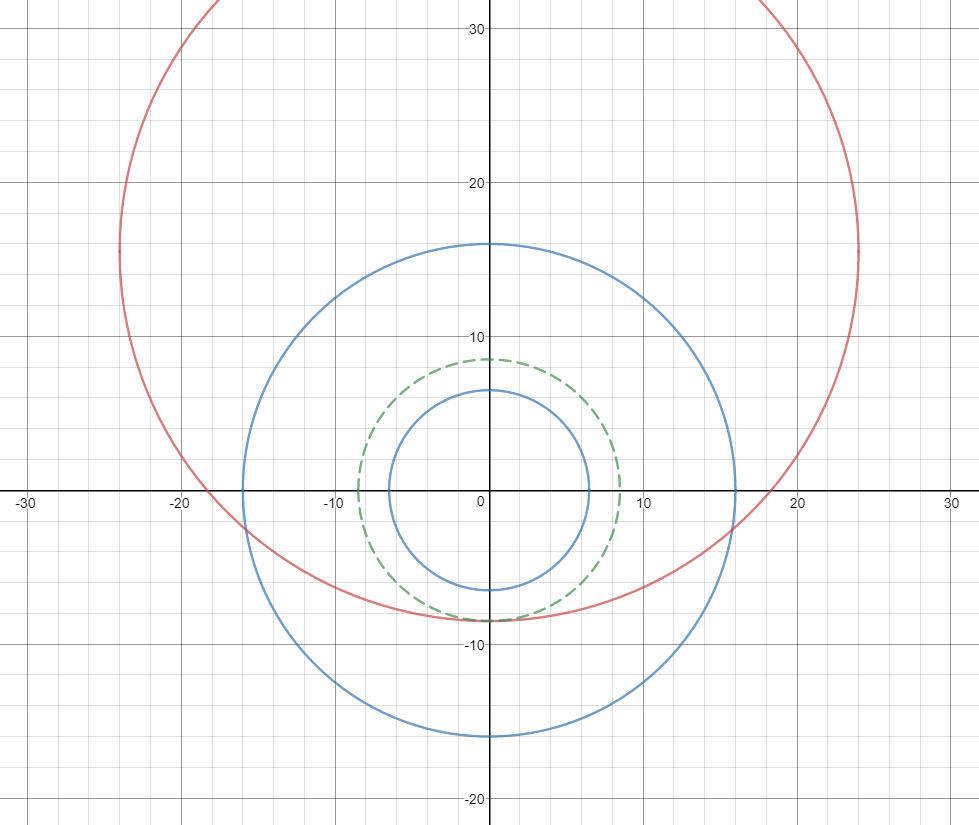
\includegraphics[width=0.32\textwidth]{Q6_diagram_1.PNG}
    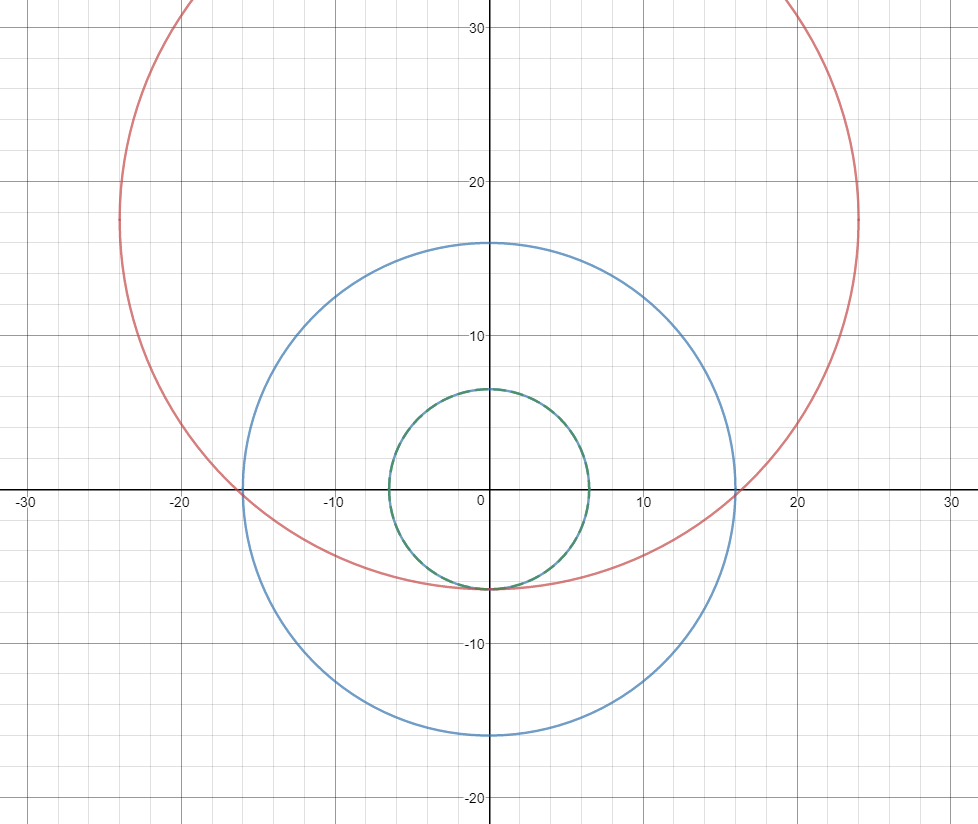
\includegraphics[width=0.32\textwidth]{Q6_diagram_2.PNG}
    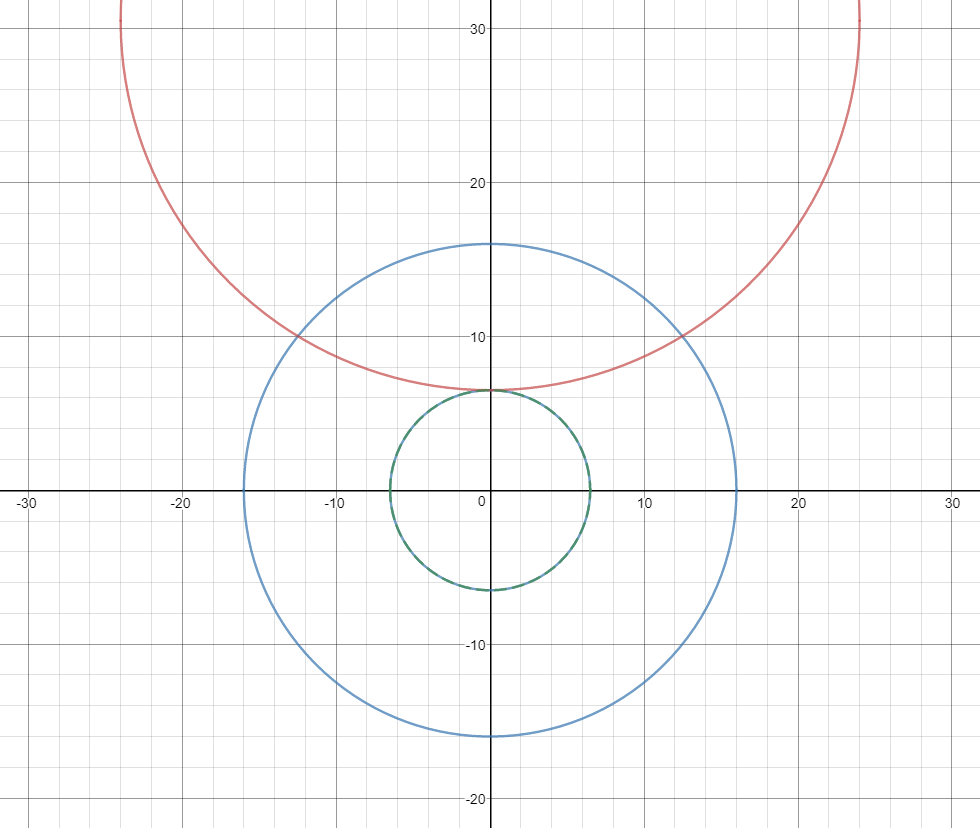
\includegraphics[width=0.32\textwidth]{Q6_diagram_3.PNG}
    \caption{Three vinyl record and tone-arm set-ups}
    \label{vinyls}
    \end{figure}
    
\item
    In my program GSS is used twice in a double iteration. The two functions being maximised/minimised are:
    \begin{itemize}
    \item \textbf{phi}, a function of $x$ for fixed $d$, which calculates $\phi$.
    \item \textbf{phiVar}, a function of $d$, which calculates $\Delta\phi$, the variance in $\phi$ as the tone-arm moves over the entirety of the record.
    \end{itemize}
    
    \begin{figure}[H]
    \centering
    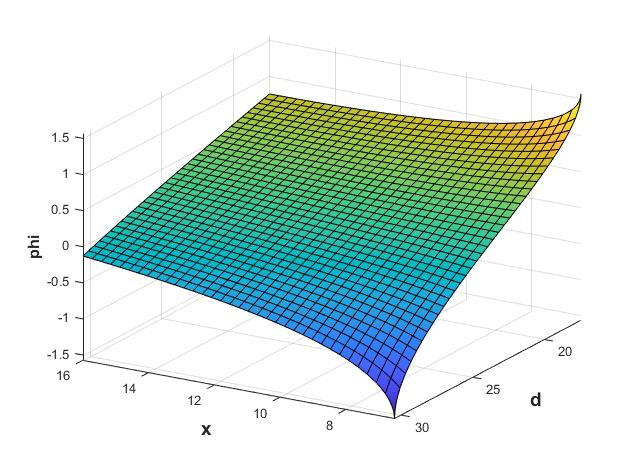
\includegraphics[width=0.60\textwidth]{Q6_ii_a.jpg}
    \caption{Surface plot of $\phi(x,d)$}
    \label{xdphi}
    \end{figure}
    
    Figure \ref{xdphi} shows a plot of $\phi$ against $x$ and $d$ on the previously specified relevant intervals of $x$ and $d$. By inspection it is clear that the cross-section of this surface with any plane perpendicular to the $d$ direction (ie fixed $d$) will be unimodal and so GSS is appropriate.
    
    \begin{figure}[H]
    \centering
    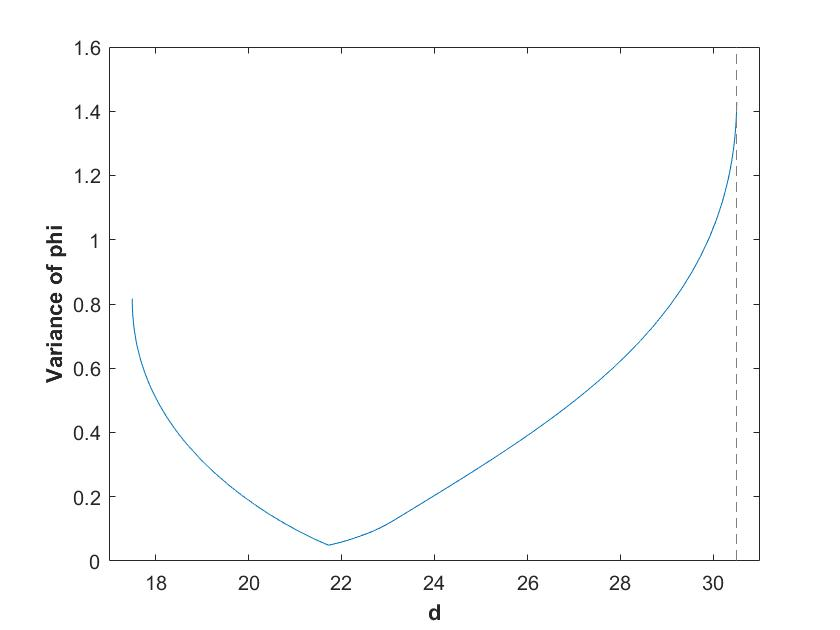
\includegraphics[width=0.60\textwidth]{Q6_ii_b.jpg}
    \caption{Plot of $\Delta\phi$ against d}
    \label{dvarphi}
    \end{figure}
    
    Figure \ref{dvarphi} shows $\Delta\phi$ against $d$ confirming that the function phiVar($d$) is unimodal over the range $17.5\leq d\leq 30.5$ and GSS is appropriate.
\item
	To find d to one decimal place 15 iterations are required:
    \begin{gather*}
    (30.5-17.5)\times(\phi^{-1})^n \leq 0.01 \\
    \Rightarrow n \geq \log_{\phi^{-1}}{0.01/13} \\
    n = 14.9 \qquad 1 dp 
    \end{gather*}
	\\
    To find $\Delta\phi$ to two decimal places 19 iterations are required:
    \begin{gather*}
    (16-6.5)\times(\phi^{-1})^n \leq 0.001 \\
    \Rightarrow n \geq \log_{\phi^{-1}}{0.001/9.5} \\
    n = 19.0 \qquad 1 dp 
    \end{gather*}
    \\
    The accuracy of my value of $d$ is dependent on the accuracy of the outer iterations (Note that the accuracy achievable is limited by the accuracy of the inner iterations if the accuracy is too large to be compare calculated d values but the inner accuracy itself doesn't contribute to the accuracy of $d$).
    \\
    The accuracy of my value of $\theta$ is dependent upon the accuracy of the inner iteration but also in directly on the accuracy of the outer iteration because the value of $d$ computed is used to calculate $\theta$.
\end{enumerate}

\pagebreak
\section*{Programs}

\subsection*{Question\textunderscore2.m}
\begin{lstlisting}[style = Matlab-editor]
a  = input('enter lower boundary: ');  % a,b - starting region
b  = input('enter upper boundary: ');
pr = input('enter precision: ');       % pr  - required precision

% decide whether uni-modal function has
%   maxima(+1) or minima(-1) or both(0) ie modes at endpoints
grada = (f(a+pr)-f( a  ))/pr;
gradb = (f( b  )-f(b-pr))/pr;
switch(sign(grada*gradb))
    case 1
        m = 0;
    case 0
        m = sign(grada+gradb);
    case -1
        m = sign(grada);
end

% If there is not a mode then print out the two end points
% Else locate the coordinate of the mode
if(m==0)
    fprintf('The equation is monotonic.\n There are two modes located at: %d, %d \n', a, b);
else
    gr = (1+sqrt(5))/2;  % Golden Ratio
    x = b - (b-a)*gr^-1;
    y = a + b - x;
    fx = f(x);
    fy = f(y);
    % iterate through Golden Sections until within required precision of the answer
    n = 0;  % counting iterations of golden section search
    while( b-a > 2*pr)
        n = n + 1;
        if(m*fx > m*fy)
            b = y;
            y = x;
            x = a+b-y;
            fy = fx;
            fx = f(x);
        elseif(m*fx < m*fy)
            a = x;
            x = y;
            y = a+b-x;
            fx = fy;
            fy = f(y);
        elseif(fx == fy)
            a = x;
            b = y;
            x = b - (b-a)*gr^-1;
            y = a + b - x;
            fx = f(x);
            fy = f(y);
        end    
    end
    X = (a+b)/2;
    fprintf('Mode located at: %d \n', X);
    fprintf('Accuracy: +/- %d \n', (b-a)/2);
end

fprintf('Number of iterations of golden section search: %d \n', n);

function[y] = f(x)
    y = 1 + x + x^2 - 4*x^4;
end

\end{lstlisting}

\pagebreak
\subsection*{Question\textunderscore6.m}
\begin{lstlisting}[style = Matlab-editor]
% restricted variables
l = 24;
r = 6.5;
R = 16;

% the precision with which to run the inner and outer golden search searches respectively
prIn  = 0.001;
prOut = 0.01;

% mode of phi(x,d) as a funciton of d
X = @(d) GSS( @(x) phi(x,d), r, R, prIn);

% variation in phi(x,d) as a function of d
%   (using the x position of mode)
phiVar = @(d) var( @(x) phi(x,d), X(d), r, R);

% locates mode of phiVar(d)
D = GSS( phiVar, l-r, l+r, prOut);

% calculates theta using dMode
theta = phi(X(D),D) + phiVar(D)/2;

fprintf("The optimum values are \n theta = %d rad \n     d = %d cm \n", theta, D);

%fsurf(@(x,d) phi(x,d),[6.5,16,17.5,30.5]);
%fplot(phiVar,[17.5,30.5]);
%axis([17,31,0,1.6]);

% function being studied
function[p] = phi(x,d)
    l = 24;
    p = pi/2 - acos( (x^2+l^2-d^2)/(2*x*l) );
end

% function calculates the variance of f with the mode of f
%    (ie the max(f)-min(f) over the range [a,b])
function[v] = var(f,mode,a,b)
    fm = f(mode);
    v = max( abs( fm - f(a) ), abs( fm - f(b) ) );
end

% Golden Section Search (GSS) w/ parameters:
%  func - function to be tested
%  a,b  - the interval boundaries
%  h    - the precision required
function[mode] = GSS(f,a,b,h)
    % check whether mode is maxima(+1) or minima(-1) or both(0)
    grada = (f(a+h)-f( a ))/h;
    gradb = (f( b )-f(b-h))/h;
    
    switch(sign(grada*gradb))
        case 1
            m = 0;
        case 0
            m = sign(grada+gradb);
        case -1
            m = sign(grada);
    end

    if(m==0)
        mode = a;
    else
        gr = (1+sqrt(5))/2;   % Golden Ratio
        A = a; B = b;         % store copies of a and b 
        x = B - (B-A)*gr^-1;
        y = A + B - x;
        fx = f(x);
        fy = f(y);
        while( B-A > 2*h)
            if(m*fx > m*fy)
                B = y;
                y = x;
                x = A+B-y;
                fy = fx;
                fx = f(x);
            elseif(m*fx < m*fy)
                A = x;
                x = y;
                y = A+B-x;
                fx = fy;
                fy = f(y);
            elseif(fx == fy)
                A = x;
                B = y;
                x = B - (B-A)*gr^-1;
                y = A + B - x;
                fx = f(x);
                fy = f(y);
            end    
        end
        mode = (A+B)/2;
    end
end

\end{lstlisting}

\end{document}





































